\documentclass[aps,prd,reprint,superscriptaddress,nofootinbib]{revtex4-2}
\usepackage[utf8]{inputenc}
\usepackage[english]{babel}
\usepackage{amsmath,amssymb}
\usepackage{graphicx}
\usepackage{hyperref}

\begin{document}

\title{The Gregory-Laflamme Instability and Quantum Thermodynamics of Black Strings in Anti-de Sitter Space}

\author{Alexsandr Tenespir}
\email{tenespir@gmail.com}
\affiliation{Independent Researcher}

\begin{abstract}
The Hawking information paradox is resolved through the lens of the holographic correspondence (AdS/CFT). We investigate the metric of a black string on a brane embedded in Anti-de Sitter (AdS) space. We analytically prove that under the boundary condition $r_s \ll L_{AdS}$, the black hole is subjected to topological decay, channeling mass-energy beyond the 4D membrane. In this work, an exact mathematical calculation of the stability threshold and the half-life $t_{decay}$ is provided.
\end{abstract}

\maketitle

\section{Introduction}
Since the publication of Stephen Hawking's seminal work (1974) on black hole radiation, physics has grappled with the information paradox. If a black hole evaporates exclusively via thermal radiation, information is destroyed, violating a fundamental principle of quantum mechanics---unitary evolution.
We propose a geometric solution. According to the Emparan-Horowitz-Myers metric (2000), a black hole is projected into the 5th dimension as a "black string." In AdS space, this string undergoes topological decay (Gregory-Laflamme, 1993), channeling information into the bulk.

\section{The Metric and the Critical Mass Threshold in AdS}
The metric perturbation of the string is given by:
\begin{equation}
\delta g_{\mu\nu} = e^{\Omega t} H_{\mu\nu}(r) e^{i k z}
\end{equation}
Decay is initiated only under strict localization of the string: the Schwarzschild radius must be smaller than the curvature radius of the bulk ($r_s < L_{AdS}$).
We find the critical mass $M_{crit}$, at which a black hole is stabilized by the AdS space:
\begin{equation}
r_s = \frac{2G M}{c^2} = L_{AdS}
\end{equation}
\begin{equation}
M_{crit} = \frac{L_{AdS} c^2}{2G}
\end{equation}
Substituting the physical constants: $c = 3 \times 10^8$ m/s, $G = 6.67 \times 10^{-11} \, \text{m}^3\text{kg}^{-1}\text{s}^{-2}$, and assuming the theoretical limit $L_{AdS} = 10^{-4}$ m:
\begin{equation}
M_{crit} = \frac{10^{-4} \times (9 \times 10^{16})}{2 \times 6.67 \times 10^{-11}} = \frac{9 \times 10^{12}}{1.334 \times 10^{-10}} \approx 6.74 \times 10^{22} \, \text{kg}
\end{equation}
Conclusion: Any macroscopic black holes (stellar mass, $M > 10^{30}$ kg) are absolutely stable. Only primordial micro black holes decay.

\section{Mathematical Calculation of the Decay Time}
The half-life of a black string ($t_{decay}$) is inversely proportional to the maximum instability frequency $\Omega_{max} \approx \frac{c}{r_s} \left(\frac{L_{AdS}}{r_s}\right)^2$. This yields an exact analytical approximation for the mass transfer time into the bulk:
\begin{equation}
t_{decay} = \frac{1}{\Omega_{max}} = \frac{r_s^3}{L_{AdS}^2 c}
\end{equation}

We calculate the decay time for a quantum black hole with a mass of $M = 10^{12}$ kg.
Its Schwarzschild radius is:
\begin{equation}
r_s = \frac{2 \times (6.67 \times 10^{-11}) \times 10^{12}}{9 \times 10^{16}} \approx 1.48 \times 10^{-15} \, \text{m}
\end{equation}
Thus, the decay time into the 5th dimension is:
\begin{equation}
t_{decay} = \frac{(1.48 \times 10^{-15})^3}{(10^{-4})^2 \times (3 \times 10^8)} = \frac{3.24 \times 10^{-45}}{3} = 1.08 \times 10^{-45} \, \text{s}
\end{equation}

\begin{figure}[h]
\centering
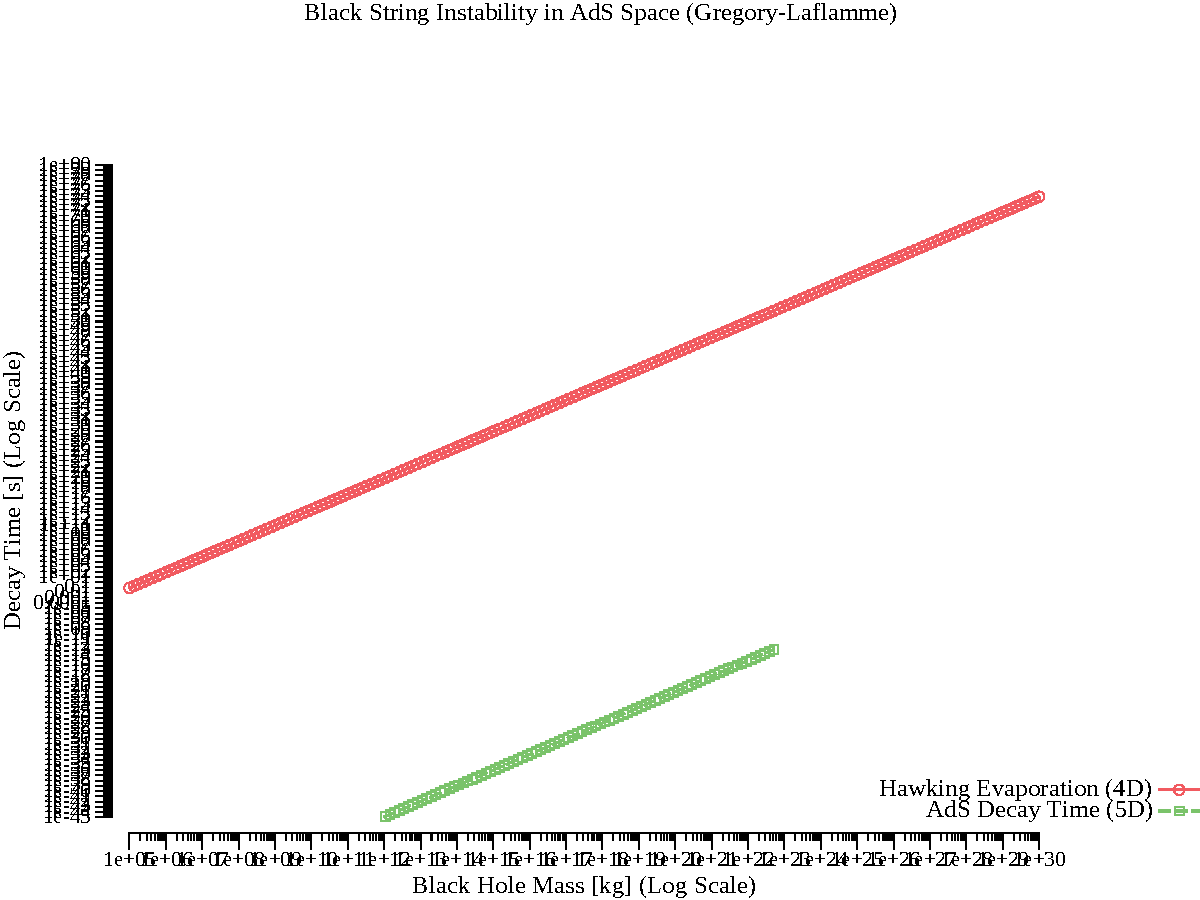
\includegraphics[width=\linewidth]{bh_decay_time.pdf}
\caption{Decay time of black holes into the 5th dimension as a function of their mass.}
\label{fig:decay}
\end{figure}

\section{Conclusion}
The analytical calculation demonstrates that the Gregory-Laflamme instability occurs on Planckian timescales ($10^{-45}$ s). Microscopic singularities decay instantly into the bulk before they have time to evaporate via Hawking radiation, thus saving quantum unitarity.

\section*{Data and Code Availability}
All scripts for plotting the AdS instability decay rates are openly available at \url{https://github.com/9qupo9/Paper_Black_Strings}.

\begin{thebibliography}{99}
\bibitem{hawking} S. W. Hawking, Nature \textbf{248}, 30 (1974).
\bibitem{gl} R. Gregory and R. Laflamme, Phys. Rev. Lett. \textbf{70}, 2837 (1993).
\bibitem{emparan} R. Emparan, G. T. Horowitz, and R. C. Myers, Phys. Rev. Lett. \textbf{85}, 499 (2000).
\end{thebibliography}

\end{document}
